\documentclass[14pt, a4paper]{article}
\usepackage[utf8]{inputenc}
\usepackage{graphicx}
\graphicspath{ {TestImages/} } 

\title{FOAR705 - Digital Humanities}
\author{Sheri Goldie}
\date{9th August 2019}

\begin{document}
\maketitle
% adding a comment to the code
Trial text editing:

To create a \underline{learning journal}, one must have two things, a \textbf{desire to learn,} and a \textit{desire to reflect on one's process for learning.}

More text to edit:

Here we shall find person's endeavouring to better themselves. \emph{It is called a university,} and should be entered with an appropriate awe. 

\textit{Here we shall find person's endeavouring to better themselves. \emph{It is called a university,} and should be entered with an appropriate awe.}

\textbf{Here we shall find person's endeavouring to better themselves. \emph{It is called a university,} and should be entered with an appropriate awe.}

To insert an image:

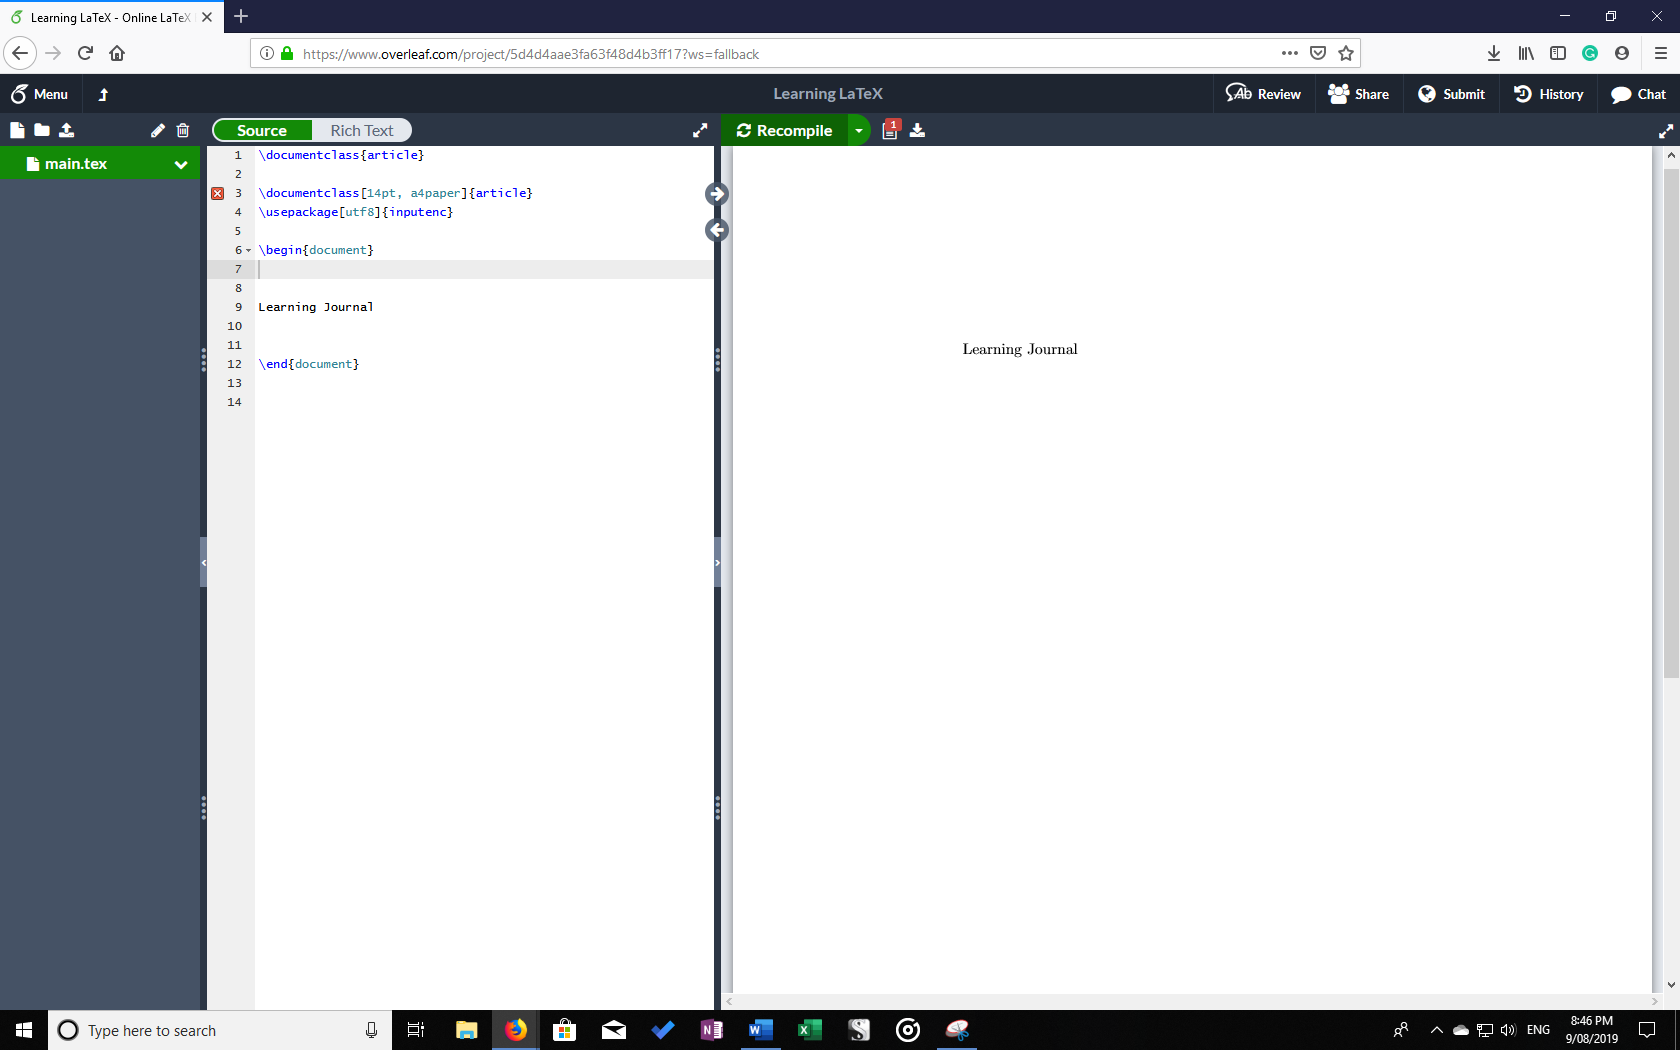
\includegraphics[width=10cm]{20190809Screenshot1.png}

\pagebreak
Or another way:
\begin{figure}[h]
    \centering
    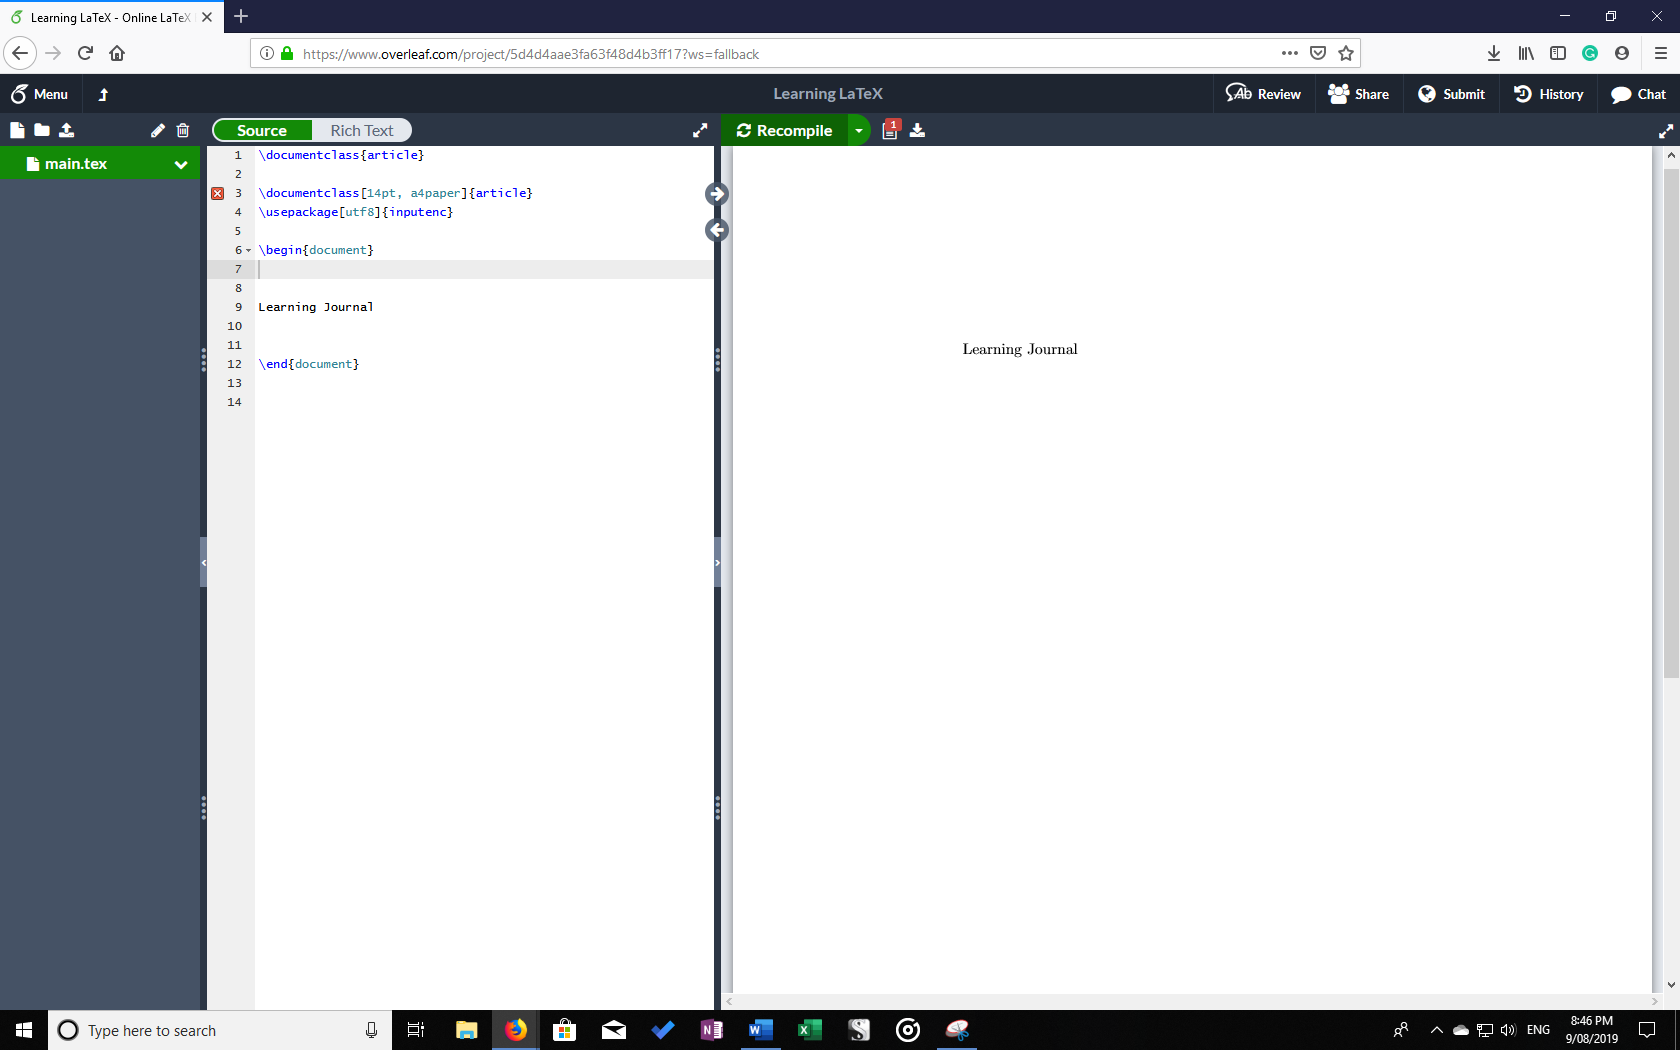
\includegraphics[width=10cm]{20190809Screenshot1.png}
    \caption{A screenshot of my first LaTeX error}
    \label{fig:screenshoterror}
\end{figure}



Inserting an image with caption references:
\begin{figure}[h]
    \centering
    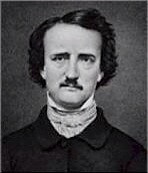
\includegraphics{poe.jpg}
    \caption{Edgar Allan Poe}
    \label{fig:PoeAuthor}
\end{figure}

In figure \ref{fig:PoeAuthor} we have Edgar Allan Poe. He also appears on page \pageref{fig:PoeAuthor} he also appears.

\pagebreak
\section{Make a List}

\textbf{Here is a list of things:}
\begin{itemize}
    \item apples
    \item oranges
    \item bananas
    \item mandarins
\end{itemize}

\subsection{List}
\textbf{Here is an ordered list of things:}
\begin{enumerate}
    \item Dogs
    \item Otters
    \item Ravens
    \item Owls
\end{enumerate}

\section{Formatting}
\begin{abstract}
This is an abstract. This section is looking at various formatting fuctions in LaTeX.
\end{abstract}

This is where new text begins.

This line will begin another paragrpah.

I can use some code
\newline
to manually create a line break.


\pagebreak

%\chapter{chapter one} and \part{part one} only works in "book" or "report" document classes
 
\section{Introduction}
 
This is the first section.
 
Lorem  ipsum  dolor  sit  amet,  consectetuer  adipiscing  
elit.   Etiam  lobortisfacilisis sem.  Nullam nec mi et 
neque pharetra sollicitudin.  Praesent imperdietmi nec ante. 
Donec ullamcorper, felis non sodales...
 
\section{Second Section}
 
Lorem ipsum dolor sit amet, consectetuer adipiscing elit.  
Etiam lobortis facilisissem.  Nullam nec mi et neque pharetra 
sollicitudin.  Praesent imperdiet mi necante...
 
\subsection{First Subsection}
Praesent imperdietmi nec ante. Donec ullamcorper, felis non sodales...
 
\section*{Unnumbered Section}
Lorem ipsum dolor sit amet, consectetuer adipiscing elit.  
Etiam lobortis facilisissem

\end{document}

